\section{Conv}
\textbf{Conv1D:} 1 boyutlu konvolüsyon işlemi uygulamak için kullanılan bir katmandır. Giriş verileri üzerinde belirli bir pencere boyutunda kaydırılan bir filtre (kernel) uygular. Bu filtre, giriş verilerini bir boyutlu konvolüsyon işleminden geçirir ve çıktı olarak konvolüsyon sonuçlarını verir. Genellikle zamansal verilerin işlenmesi, sıralı verilerin analizi gibi durumlarda kullanılır.\\
\textbf{Conv2D:} 2 boyutlu konvolüsyon işlemi uygulamak için kullanılan bir katmandır. Giriş verileri üzerinde belirli bir pencere boyutunda kaydırılan bir filtre (kernel) uygular. Bu filtre, giriş verilerini iki boyutlu konvolüsyon işleminden geçirir ve çıktı olarak konvolüsyon sonuçlarını verir. Genellikle görüntü işleme gibi iki boyutlu verilerin işlenmesi durumlarda kullanılır. \\
\textbf{Conv3D:} 3 boyutlu konvolüsyon işlemi uygulamak için kullanılan bir katmandır. Giriş verileri üzerinde belirli bir pencere boyutunda kaydırılan bir filtre (kernel) uygular. Bu filtre, giriş verilerini üç boyutlu konvolüsyon işleminden geçirir ve çıktı olarak konvolüsyon sonuçlarını verir. Genellikle video işleme, 3D görüntü verileri gibi üç boyutlu verilerin işlenmesi durumlarda kullanılır.

\begin{figure}[h]
    \centering
    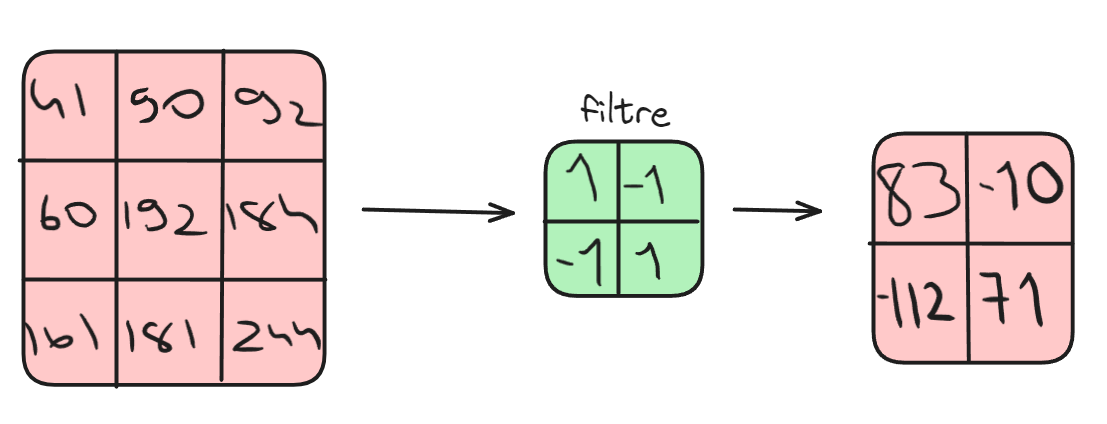
\includegraphics[width=0.7\textwidth]{images/conv_layer.png}
    \caption{Konvolüsyon katmanı.}
    \label{fig:enter-label}
\end{figure}

\subsubsection{Hiperparametreler}
\begin{table}[h]
\centering
{\scriptsize\renewcommand{\arraystretch}{0.4}
{\resizebox*{\linewidth}{0.2\textwidth}{
\begin{tabular}{|p{2cm}|p{6cm}|}
\hline
Parametre & Açıklama \\ \hline
filters & Çıkış uzayının boyutu. \\ \hline
kernel\_size & Filtre boyutu. \\ \hline
stride & Kaydırma adımı \\ \hline
padding & Giriş boyutunu ayarlamak için kullanılcak yöntem. \\ \hline
activation & Aktivasyon fonksiyonu. \\ \hline

\end{tabular}
}}}
\end{table}

\newpage

\subsection{Separable Convolution}

Separable Convolution, klasik konvolüsyon katmanının iki aşamaya bölünmesiyle elde edilen bir işlemdir. Normal bir konvolüsyon işlemi, giriş görüntüsüne filtre uygularken aynı anda hem uzaysal (spatial) hem de kanal (depth) boyutunda bir ağırlıklandırma yapar. Ancak bu işlem yüksek hesaplama maliyetine sahiptir. Separable Convolution bu işlemi iki ayrı adıma ayırır:

\begin{itemize}
    \item \textbf{Depthwise Convolution}: Girişteki her kanala ayrı ayrı bir filtre uygular. Yani, bir filtre yalnızca kendi kanalındaki piksellere uygulanır.
    \item \textbf{Pointwise Convolution}: Bu aşama 1x1 boyutunda filtreler kullanarak her pikselin her kanalında bir ağırlıklandırma yapar ve sonuçları kanallar arasında birleştirir.
\end{itemize}

Giriş görüntü boyutları $H \times W \times D$ (yükseklik, genişlik, kanal sayısı) ve normal konvolüsyonda kullanılan filtrelerin boyutları $K \times K \times D \ times N$ (filtre yüksekliği, genişliği, giriş kanalı, çıkış kanalı) ise normal bir konvolüsyonda gereken hesaplama yükü:

\[ H \times W \times K \times K \times D \times N \]

Ancak Separable Convolution da bu işlem iki aşamaya bölünerek şu hale gelir.

\begin{enumerate}
    \item \textbf{Depthwise Convolution}: $H \times W \times K \times K \times D$
    \item \textbf{Pointwise Convolution}: $H \times W \times D \times N$
\end{enumerate}

\newpage